% Walter Wißdorf, Minimal PGF Plots exame

% Document Header / Configuration -------------------------------------------------------------------------------------
\documentclass[a4paper,titlepage,DIV11,11pt,BCOR2.5cm,headinclude,english,openany,pdftex]{scrbook}

% encoding, babel
\usepackage[utf8]{inputenc}
\usepackage{babel}
\usepackage{babelbib} 

% Images / floats


\usepackage{xspace}
\usepackage[final]{graphicx}
\usepackage{units}

%"dynamic" graphics packages section................
%tikz configuration
\usepackage{tikz}
\usetikzlibrary{arrows}
\usepackage{gnuplottex} %plotting of analytical functions with gnuplot
\usepackage{pgfplots} %tikz based plotting package
\usepackage{calc} %for length calculations
% ..................................................

% Change font styles
\usepackage{fourier}
\usepackage{sectsty}
\allsectionsfont{\fontfamily{phv}\selectfont} 
\tolerance=300


% new commands / macros
\newcommand{\mobUnit}{$10^{-4} \mathrm{m}^2 \mathrm{V}^{-1} \mathrm{s}^{-1}$} %used ion mobility unit
\newcommand{\inMobUnits}[1]{\unit[#1]{$\cdot$\mobUnit}} %macro for mobility unit with value


% ----- define some standard colors with systematic names for graphics in the document -------
\definecolor{cffffff}{RGB}{255,255,255}
\definecolor{caaeeff}{RGB}{170,238,255}
\definecolor{c0080cc}{RGB}{0,128,204}
\definecolor{cl1_dark}{RGB}{253,103,17} 	%dark oragne
\definecolor{cl1_light}{RGB}{253,170,115} 	%light orange
\definecolor{cl2_dark}{RGB}{32,103,170} 	%dark blue
\definecolor{cl2_light}{RGB}{203,227,247} 	%light blue
\definecolor{cl3_dark}{RGB}{253,26,18} 	%dark red
\definecolor{cl3_light}{RGB}{254,128,124} 	%light red
\definecolor{cl4_dark}{RGB}{29,121,1} 	%dark green
\definecolor{cl4_light}{RGB}{156,254,139} 	%light green


% ----- define some standard lengths with systematic names for graphics in the document -------
\newlength{\singleplotwidth}
\setlength{\singleplotwidth}{\columnwidth *\real{0.7}}
\newlength{\singleplotheight}
\setlength{\singleplotheight}{\singleplotwidth *\real{0.8}}

\newlength{\largesingleplotwidth}
\setlength{\largesingleplotwidth}{\columnwidth *\real{1.0}}
\newlength{\largesingleplotheight}
\setlength{\largesingleplotheight}{\largesingleplotwidth *\real{0.70}}


\newlength{\doubleplotwidth}
\setlength{\doubleplotwidth}{\columnwidth *\real{0.6}}
\newlength{\doubleplotheight}
\setlength{\doubleplotheight}{\doubleplotwidth *\real{0.9}}






%------------------------------------------ DOC START ------------------------
\begin{document}


% ----- now the main part / main text

\begin{figure}[!tb]
   \begin{center}
   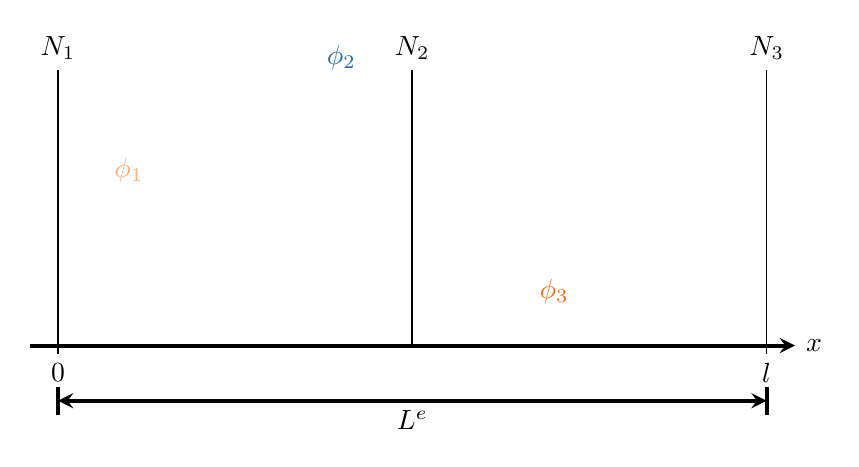
\begin{tikzpicture}[domain=0:1,x=9cm,y=3.5cm,scale=1]
	\tikzset{>=stealth}
	\tikzstyle{line} = [line width=1.4pt]
	\tikzstyle{thinline} = [line width=0.6pt]

	%plots....
    \draw[line,color=cl1_light] plot[id=phi1,samples=100] function{(1-x)*(1-2*x)};
    \draw[line,color=cl1_light] (0.1,0.72) node[below] {$\phi_1$};

    \draw[line,color=cl2_dark,dashed] plot[id=phi2,samples=100] function{4*x*(1-x)};
    \draw[line,color=cl2_dark] (0.4,0.96) node[above] {$\phi_2$};
        
    \draw[line,color=cl1_dark,densely dotted] plot[id=phi3,samples=100] function{x*(2*x-1)};
	\draw[line,color=cl1_dark] (0.7,0.28) node[below] {$\phi_3$};

	%baseline and node positions....        
    \draw[line,->] (-0.04,0) -- (1.04,0) node[right] {$x$};
    \draw[thinline,-] (0,0) -- (0,1) node[above] {$N_1$};
    \draw[thinline,-] (0.5,0) -- (0.5,1) node[above] {$N_2$};
    \draw[thinline,-] (1,0) -- (1,1) node[above] {$N_3$};

	%baseline annotations....
	\draw (0,1pt) -- (0,-3pt) node[anchor=north] {$0$};
    \draw (1,1pt) -- (1,-3pt) node[anchor=north] {$l$};

	%L^e annotation....    
    \draw[line,<->] (0,-0.2) -- (1,-0.2);
    \draw (0.5,-0.2) node[anchor=north] {$L^e$};
    \draw[line,-] (0,-0.25) -- (0,-0.15);
    \draw[line,-] (1,-0.25) -- (1,-0.15);

\end{tikzpicture}
   \caption{Example of analytical one dimensional shape function plots (requires gnuplot)}
   \label{fig:1d-shape-functions}
   \end{center}
\end{figure}

% Figure: Ion migration (IMS Pot): Simion simulated ion current, comparison of turbulent and laminar results
\begin{figure}[!tb]
   \begin{center}
   %plot velocity / mobility comparision

\begin{tikzpicture}[scale=1]
	\tikzstyle{line} = [line width=1.2pt, mark options=solid]
	\tikzset{every mark/.append style={scale=1.2}}

	\begin{axis}[
        ymin=0,ymax=1.0, 
        %xmin=0,xmax=20,
        xlabel=deflection voltage (\unit{V}),
        ylabel=relative ion current (arbitrary units),
        width=\largesingleplotwidth,
        height=\largesingleplotheight,
        legend style={
            %area legend,
            at={(0.5,-0.19)},
            anchor=north,
            legend columns=2,
            cells={anchor=west}
            } 
        ]


    \addplot[cl1_dark,mark=o,line]               table[col sep=comma,x index=0,y index=2] {data/simion/sim2012_12_05_001.csv}; 
    \addplot[cl1_dark,mark=o,line, dashed]       table[col sep=comma,x index=0,y index=2] {data/simion/sim2012_12_02_001.csv}; 
    \addplot[cl2_dark,mark=diamond,line]         table[col sep=comma,x index=0,y index=2] {data/simion/sim2012_12_05_002.csv}; 
    \addplot[cl2_dark,mark=diamond,line, dashed] table[col sep=comma,x index=0,y index=2] {data/simion/sim2012_12_02_002.csv}; 
    \addplot[cl3_dark,mark=asterisk,line]        table[col sep=comma,x index=0,y index=2] {data/simion/sim2012_12_05_003.csv}; 
    \addplot[cl3_dark,mark=asterisk,line,dashed] table[col sep=comma,x index=0,y index=2] {data/simion/sim2012_12_02_003.csv}; 
    \addplot[cl4_dark,mark=asterisk,line]        table[col sep=comma,x index=0,y index=2] {data/simion/sim2012_12_05_004.csv}; 
    \addplot[cl4_dark,mark=asterisk,line,dashed] table[col sep=comma,x index=0,y index=2] {data/simion/sim2012_12_02_004.csv}; 


    %\addplot[cl2_dark,mark=asterisk,line] table[col sep=comma,x index=0,y index=1] {data/deflectVari_negCorona-posDeflect_1-1SLM.csv};
        
    \legend{
        {\unit[0.45]{m/s}, laminar},
        {\unit[0.45]{m/s}, turbulent},
        {\unit[0.65]{m/s}, laminar},
        {\unit[0.65]{m/s}, turbulent},        
        {\unit[0.85]{m/s}, laminar},
        {\unit[0.85]{m/s}, turbulent},
        {\unit[1.35]{m/s}, laminar},
        {\unit[1.35]{m/s}, turbulent},
    };
    \end{axis}
\end{tikzpicture}
   \caption{\emph{SIMION simulation results:} Effects of the turbulence model on the simulated ion current on the receiver electrode. The general shape of the simulated ion current response on the deflection voltage without turbulence modeling ("laminar") and with $k-\epsilon$ turbulence model ("turbulent") is similar but with turbulence modeling the effect of the gas flow is significantly more pronounced.}
   \label{fig:ionMigSim-simion-turbulent-laminar}
   \end{center}
\end{figure}

% Figure: Ion migration (IMS Pot): Simion simulated ion current, comparison with experimental result
\begin{figure}[!tb]
   \begin{center}
   %plot velocity variation

\begin{tikzpicture}[scale=1]
	\tikzstyle{line} = [line width=1.0pt, mark options=solid]
	\tikzset{every mark/.append style={scale=1.8}}

	\begin{axis}[
        name=leftPlot,
        ymin=0,ymax=1.0, 
        xmin=0,xmax=20, 
        xlabel=deflection voltage (\unit{V}),
        ylabel=relative ion current (arbitrary units),
        width=\doubleplotwidth,
        height=\doubleplotheight,
        legend style={
            %area legend,
            at={(1,-0.19)},
            anchor=north,
            legend columns=2,
            cells={anchor=west}
            }
        ]


    \addplot[cl1_dark,mark=o,line]        table[col sep=comma,x index=0,y index=2] {data/simion/sim2012_12_02_001.csv}; 
    \addplot[cl1_dark,mark=triangle,line] table[col sep=comma,x index=0,y index=2] {data/simion/sim2012_12_02_002.csv}; 
    \addplot[cl1_dark,mark=star,line]     table[col sep=comma,x index=0,y index=2] {data/simion/sim2012_12_02_003.csv}; 
    \addplot[cl1_dark,mark=diamond,line]  table[col sep=comma,x index=0,y index=2] {data/simion/sim2012_12_02_004.csv}; 
    \addplot[cl2_dark,mark=square*,line]  table[col sep=comma,x index=0,y index=2] {data/experimental/ww_2012_12_13_02.xls_analyzed.csv}; 
    \addplot[cl2_dark,mark=*,line]        table[col sep=comma,x index=0,y index=2] {data/experimental/ww_2012_12_13_03.xls_analyzed.csv}; 


    %\addplot[cl2_dark,mark=asterisk,line] table[col sep=comma,x index=0,y index=1] {data/deflectVari_negCorona-posDeflect_1-1SLM.csv};
    \legend{
        {simulation, \unit[0.45]{m/s}},
        {simulation, \unit[0.65]{m/s}},
        {simulation, \unit[0.85]{m/s}},
        {simulation, \unit[1.25]{m/s}},
        {measurement, \unit[0.35]{m/s}},
        {measurement, \unit[0.45]{m/s}},
    };


    \end{axis};

    \begin{axis}[
        ymin=0,ymax=1.0, 
        xlabel=deflection voltage (\unit{V}),
        %ylabel=relative ion current (arbitrary units),
        yticklabels={,,}, %hide y ticks 
        width=\doubleplotwidth,
        height=\doubleplotheight,
        at={(\doubleplotwidth*0.8,0)}, anchor=left of south west,
        legend style={
            %area legend,
            at={(1,-0.19)},
            anchor=north,
            legend columns=2,
            cells={anchor=west}
            }
        ]

    \addplot[cl1_dark,mark=o,line]        table[col sep=comma,x index=0,y index=2] {data/simion/sim2012_12_02_001.csv}; 
    \addplot[cl1_dark,mark=triangle,line]    table[col sep=comma,x index=0,y index=2] {data/simion/sim2012_12_02_002.csv}; 
    \addplot[cl1_dark,mark=star,line]      table[col sep=comma,x index=0,y index=2] {data/simion/sim2012_12_02_003.csv}; 
    \addplot[cl1_dark,mark=diamond,line]  table[col sep=comma,x index=0,y index=2] {data/simion/sim2012_12_02_004.csv}; 
    \addplot[cl2_dark,mark=square*,line]    table[col sep=comma,x index=0,y index=2] {data/experimental/ww_2012_12_13_02.xls_analyzed.csv}; 
    \addplot[cl2_dark,mark=*,line]      table[col sep=comma,x index=0,y index=2] {data/experimental/ww_2012_12_13_03.xls_analyzed.csv}; 

    %\addplot[cl2_dark,mark=asterisk,line] table[col sep=comma,x index=0,y index=1] {data/deflectVari_negCorona-posDeflect_1-1SLM.csv};
        
    \end{axis};

\end{tikzpicture}
   \caption{\emph{SIMION simulation results:} Simulated ion current on the receiver electrode for different bulk gas flow velocities in comparison to the experimentally determined ion current. The masses of the simulated ions was uniformly distributed between \unit[$19-350$]{Da} (estimated \inMobUnits{$K_0=3.56-1.04 $})}
   \label{fig:ionMigSim-simion-velocity}
   \end{center}
\end{figure}


\end{document}
%----------------------------------------------------------------------------